\documentclass{article}
\usepackage[utf8]{inputenc}
\usepackage{amsmath}
\usepackage{amssymb}
\usepackage{textcomp,gensymb}
\usepackage{todonotes}
\usepackage{hyperref}
\hypersetup{
    colorlinks = true,
    urlcolor = blue,
    citecolor = black
} 
\usepackage[bottom=2cm, right=3cm, left=3cm, top=1.5cm]{geometry}
\usepackage{cancel}
\usepackage{physics}
\usepackage{graphicx}
\graphicspath{ {./images/} }
%\begin{center}\includegraphics[scale = 0.25]{name}\end{center}
\newcommand{\R}{\mathbb{R}}
\newcommand{\Z}{\mathbb{Z}}
\newcommand{\qed}{\qquad${}$\hfill$\square$\\}
\newcommand{\qqR}{\qquad\Rightarrow\qquad}
\newcommand{\qqand}{\qquad\text{and}\qquad}
\newcommand{\qqor}{\qquad\text{or}\qquad}
\newcommand{\qiff}{\quad\Longleftrightarrow\quad}
\newcommand{\qqiff}{\qquad\Longleftrightarrow\qquad}
\newcommand{\qqiffdf}{\qquad\Longleftrightarrow_{df}\qquad}
\renewcommand{\b}[1]{\boldsymbol{#1}}

\title{Midterm Checkpoint}
\author{Group 11: Kevin Hefner, Shri Lekkala, YingTing Lu}
\date{November 14th, 2023}
\begin{document}
\maketitle


\subsection*{1. Introduction}
Complex ecosystems and precise inter-species dynamics can often be simplified down to a straightforward food web, delineating predators and their prey. To understand how populations of different animals ebb and flow through seasons, we may wish to simulate this predation, to better understand the dynamics of the ecosystem over time. Our project serves to implement three different approaches to modeling the predator-prey dynamics that can arise when a third animal, a superpredator that preys on all others, is introduced to a living environment. \cite{cats_protecting_birds,cats_protecting_revisited} Our three models of this “superpredator release” are simply described as follows:\begin{enumerate}
    \item First, we implement a model that utilizes the Lotka-Volterra equations \cite{meiss_textbook}:
    $$\begin{cases}
        \dv{A}{t} = r_0A\qty(1-\frac{A}{K}) - \mu_0AB - \nu_0AC\\
        \dv{B}{t} = -r_1B + \mu_1AB - \eta_0BC\\
        \dv{C}{t} = -r_2C + \nu_1AC + \eta_1BC
    \end{cases}$$
    \indent (for an explanation of the terms of these equations, see \textbf{2. Notation} below.)\\
    These differential equations give a simple way to simulate all interactions between prey, predators, and superpredators, in a continuous timespan. These equations exist under many assumptions to give them a far simpler, form but these assumptions do not incongruously limit the breadth of behavior that is visible.
    \item Next, we look to model the actions of individual animals through a non-spatial agent model. This simulates each animal as an independent actor, with uniform probability of interaction between all agents.
    \item Finally, while this has not yet been implemented, we plan to expand our project by implementing a spatial agent model. With model, we tackles the shortcoming of the uniform probability of interaction that is present in the non-spatial agent model. Here, we model animals as individuals agents, but in such a way that agents are only capable of interacting with other agents that are "close enough" to them. The simulation of each agent is informed by its position, and the identity of agents in surrounding grid-positions.
\end{enumerate}
\indent With these three models, we hope to gain a perspective on issues and advantages in each. As with any complex process that is too difficult to model exactly, the choice of model is a crucial step so that important features are highlighted and unimportant features can be safely ignored.

\subsection*{2. Numerical Methods, Packages, and Notation}
While our first and second models are vastly different in implementation and form, they use a mostly overlapping set of packages. Throughout every model, we heavily use \verb|numpy|, to more easily work with arrays of values. For example, our ODE model utilizes \verb|numpy| arrays to hold our resulting simulation populations over time, and our non-spatial agent model uses \verb|numpy|. We additionally use \verb|matplotlib.pyplot| throughout for plotting our results. The code that utilizes this packages is mostly constrained to either of the \verb|plot| functions in our two implemented models, and these are the only functions that require any plotting to be done. Finally our ODE model requires some numerical ODE approximation, which in our case, was done with \verb|scipy.integrate.solve_ivp|.\par
To best explain the numerical methods present in our project we wish to investigate the two implement models separately.\begin{itemize}
    \item Our ODE model requires the numerical solution to an ordinary differential equation in three dimensions, and as explained above, this is being done with \verb|scipy.integrate.solve_ivp|. Note that this function, without further configuration is unable to model the release of our superpredators at the parameterized release-time, so we instead run our ODE-solver in two steps. First, by running with only populations of the prey and predator, we use the ODE solver in its simplest configuration. Next, we pause the solver and instantaneously change the superpredator population at the termination of our first step to be the desired number. This 3-tuple of populations then serves as our new initial populations, as we again run the ODE-solver to finish the desired time-interval, but not note that we are simulating the changes in population of all three species. The output of \verb|scipy.integrate.solve_ivp| gives all the information needed to visualize the model's simulation, and thus our model is completed.
    \item In our non-spatial agent model, we do not require any complex numerical method, because we have instead used object-oriented programming to hold the desired features and information of all of our agents \cite{Agents.jl}. Using our \verb|Nonspatial_Agent| object, we can simply construct lists of agents and iterate through these lists in each iteration in order to simulate hunting, reproduction, the passage of time, and death. We have divided each iteration be ran by calling a method, and this allows for readability of the code that organizes how iterations are computed before and after the superpredator release.
\end{itemize}

Finally, we must explain the notation we have used throughout. We have signified the three species by $A$, $B$, and $C$, so that species $A$ is the prey, $B$ is the predator (aka the mesopredator), and $C$ is the superpredator. There is no further notation used in the agent models, but we need to explain the great number of parameters present in our Lotka-Volterra equations.\par
The Lotka-Volterra equations we use, tailored for three species, are:
$$\begin{cases}
    \dv{A}{t} = r_0A\qty(1-\frac{A}{K}) - \mu_0AB - \nu_0AC\\
    \dv{B}{t} = -r_1B + \mu_1AB - \eta_0BC\\
    \dv{C}{t} = -r_2C + \nu_1AC + \eta_1BC
\end{cases}$$
Each of $r_0,r_1,r_2,\mu_0,\mu_1,\nu_0,\nu_1,\eta_0,\eta_1$ is a parameters that determines how the different species interact, with their choice of variable-letter signifying what process they refer to:\begin{itemize}
    \item $r_0,r_1,r_2$ are all growth rates --- $r_0$ is the growth rate of the prey, and $r_1,r_2$ are death rates of the predator and superpredator.
    \item $K$ signifies the carrying capacity of the environment, the maximum number of prey animals that can exist before their growth turns negative, as if they are dying of overpopulation.
    \item $\mu_0,\mu_1$ describe the hunting relationship between species $A$ and $B$, with $A$ being hunted at some rate $\mu_0$, and species $B$ gaining in population by some rate $\mu_1$ because of this hunting.
    \item $\nu_0,\nu_1$ describe the hunting relationship between species $A$ and $C$, equivalently as to $\mu_0,\mu_1$.
    \item $\eta_0,\eta_1$ describe the hunting relationship between species $B$ and $C$, equivalently as to $\mu_0,\mu_1$.
\end{itemize}
This concludes the notation used in the first two models of our project.

\subsection*{3. Structure of \textbackslash src\textbackslash\;Folder}
As we plan to have three models, each with its own contained behavior and methods, we will be writing each model as a class, so that when the user instantiates an instance of that class, the model is constructed and finished all computations at initialization. Thus, our \verb|\src\| folder contains three \verb|.py| files, one for each method. We plan to further have that the spatial model will inherit from the non-spatial model, and the same will apply the spatial agent and non-spatial agent classes. Making each model its own file in \verb|\src| allows for code to be constructed and modified without effecting other models, and keeps all functions needed for one model in one file for readability.\par
There are two more files present in the \verb|/src/| folder: \verb|tools.py|, which contains some common functions used to validate inputs; and \verb|__init__.py| which exists to define the variable \verb|__all__|, so that importing $\ast$ works as intended.

\subsection*{4. Tests and Code Validation}
Currently there are two test files in the test folder: \verb|test_nonspatial_agent_model.py| and \\
\verb|test_ode_model.py|. These tests are built using the python \verb|unittest| framework and they can run by navigating to the \verb|\src\| directory and using the command "\verb|python -m unittest|". Across the two files there are 20 unittests which all pass. \par
The primary aim of the tests is to ensure that the input validation for each model class is working as expected. For each possible user inputted parameter of the model, the tests check that an "invalid" input is correctly identified and that the corresponding error is raised with the appropriate error message. 
For example, for the parameter \verb|N_release| in the \verb|Nonspatial_Agent_Model| class, there are tests to ensure that an incorrect input is caught. Specifically, \verb|N_release| must be an integer, and must be between 0 and "n\_steps", if this is not the case, the model will not be constructed.
The advantage of this is that if a user incorrectly or unknowingly inputs a invalid value, then they will know exactly what to modify in order to get the model working as expected. \par
Further, we plan to implement more tests for the final project that will ensure that all the models are working as expected (either deterministically, or with an element of randomness), given a set of fixed initial conditions.

\subsection*{5. Preliminary Investigations and Evaluations}
As our model's parameter cannot be directly compared to easily measurable constants in the real world, we lack any data to compare our model's results to. Thus, instead of comparing our results to some "ground truth" result, we instead wish to  consider various parameter sets that yield unique and interesting behavior.\par
Models 1, 2, and 3 below are creating using the ODE method and Lotka-Volterra equations, while Model 4 utilizes our non-spatial agent method, exhibiting more randomness and a clear jagged plot.\begin{enumerate}
    \item${}$\\
    \centerline{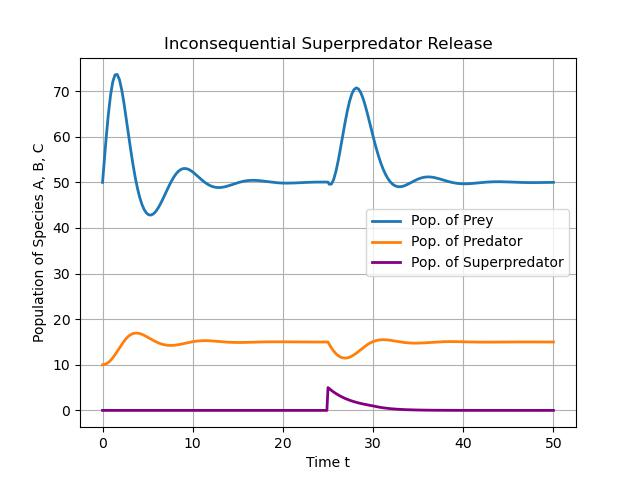
\includegraphics[scale=0.7]{images/inconsequential.jpg}}\\
    This model employed a common setting where the prey (species A) exhibited the highest fecundity and was preyed upon by two other species simultaneously (species B and superpredator C). Species B had already reached ecological equilibrium with species A before the emergence of super-species C. In this scenario, the populations of species A and B tended to stabilize under the current parameter setting.\par
    Upon the introduction of super-species C, due to the higher value of species B as prey, species C exhibited a preference for preying on species B. This led to a significant decline in the population of species B. Simultaneously, the population of species A increased due to the decrease in species B. However, after a certain period, the populations of the three species reached equilibrium.\par
    A real-world example illustrating a similar ecological dynamic is the case of the Cane Toad, originally from South and Central America. Introduced into Australia in the early 20th century to control beetles and insect pests in fields, the Cane Toad quickly adapted to the local environment and spread across Australia. \cite{Invasive_toads} Initially posing a threat to native flora and fauna due to their toxin secretion, over time, some local predators learned to avoid the toads or developed tolerance to the toxin, resulting in the establishment of a new ecological balance.
    \item${}$\\
    \centerline{\includegraphics[scale=0.7]{images/mesopred_replacement.jpg}}\\
    In the mesopredator replacement scenario, we modeled a superpredator favoring species B, forcing the predator species into extinction and allowing the superpredators to fill the predator ecological niche.\par
    This mirrors the real-world example of Brown Tree snakes in Guam, where the introduction of the superpredator led to the near extinction of native bird species (analogous to species B), establishing a new ecological equilibrium between the introduced predator and remaining native species. \cite{ecology_of_fear}
    \item${}$\\
    \centerline{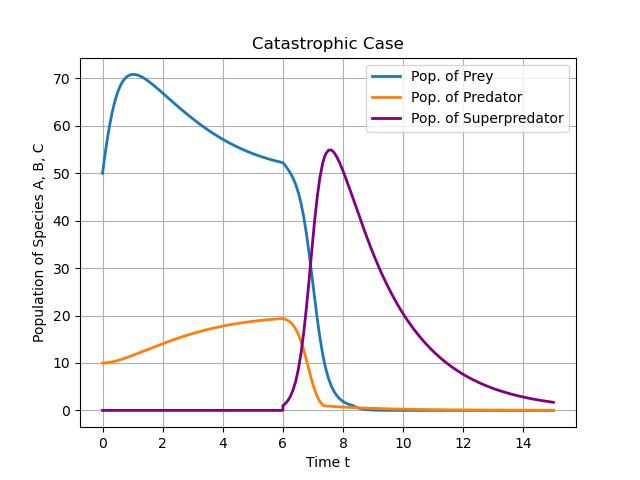
\includegraphics[scale=0.7]{images/catastrophic.jpg}}\\
    Here, we have located a set of parameters that causes the extinction of all species after the release of the superpredators. This occurs in our model, as the superpredators gain too much in population from hunting the large number of prey available. This spikes the superpredator population to a point that they quickly eliminate all prey and predators. Finally, the superpredators go extinct as they lack any food source.\par
    This situation is not easily paralleled in the real-world, but this does highlight another use of our model. One could work to model a real situation of prey and predators, and then test various superpredator release populations to ensure that this case is not experience in a real ecosystem.
    \item${}$\\
    \centerline{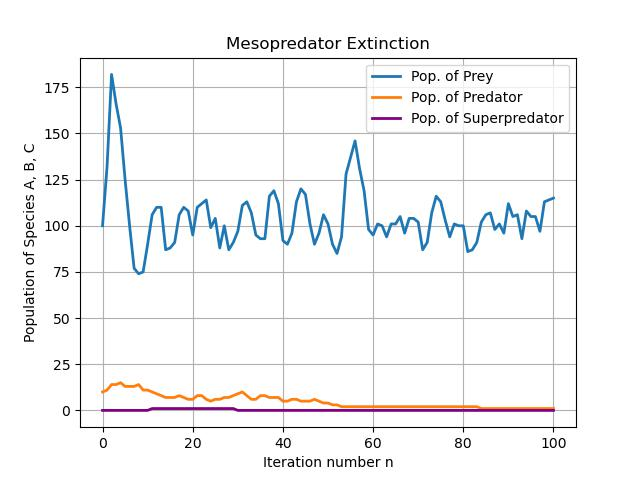
\includegraphics[scale=0.7]{images/mesopred_extinction.jpg}}\\
    Finally, we consider a model using our non-spatial agent model. We immediately see that our populations are more jagged, as this model only consider integer units of population and no decimals. We can better see the randomness exhibited in reproduction and hunting, which is not present in the Lotka-Volterra model.\par
    The situation we have modelled is that in which even the release of a single superpredator destroys the ecosystem by causing the mesopredator and superpredator to extinct. This is not however, the catastrophic case, as prey species A remains after mesopredator and superpredator extinction. We could see this situation in the real-world when a non-native species invades an ecosystem leading to destabilization.
\end{enumerate}

\subsection*{6. Proposed Variations and Improvements}
There are several extensions that we are currently considering for the final project:
\begin{enumerate}
    \item Adding a Spatial Agent model. --- We are most determined to add this variation to the non-spatial agent model, and this will be our most immediate point-of-focus in the coming days.\begin{enumerate}
        \item Using a spatial agent model would allow us to take into account the spatial dynamics of predator and prey systems, and thus will be more representative of real life. By simulating the interactions of the predator, prey, and superpredator species in a 2D space, we hope to be able to see packs form, and the 2D grid we create being divided in some sense, into regions that are dominated by each species.
        \item We would add this model class to the file \verb|spatial_agent_model.py|, which we will be able to explore and compare against our existing models. This class will most definitely inherit from the \verb|Nonspatial_Agent_Model|, as many of their methods will have the same form, but with slightly different behavior. We will also create a \verb|Spatial_Agent| class, inheriting from \verb|Nonspatial_Agent|, that is modified to also include the agent's $x,y$ position as an instance variable.
        \item This spatial agent will not require any data, as we only need parameters on which to run the model, which can be chosen at random, with some careful trial and error to find the final crucial parameters.
        \item The construction of this code will take inspiration from "Agents.ji" an agent-modeling package for Julia, but will be our own implementation due to the obvious difference in coding language. \cite{Agents.jl}
    \end{enumerate}
    \item Visualizing and Animating the Spatial Agent model.\begin{enumerate}
        \item After implementing our spatial agent model, we would aim to create visualizations of change in spatial dynamics over time. By doing so, we would be able to investigate if there are any conditions that arise to systems which exhibit oscillatory behavior in 2d space, and again to consider the visual features of a given model that give rise to particular long-term behavior.
        \item This may be done by expanding upon the plot feature in our model class. As demonstrated in lecture, we plan to use \verb|matploblib.pyplot.FuncAnimation| to animate our model, and to provide video files that can be replayed. \cite{Goodwill}
        \item This extension would again require no data, it would only be a new function added to the \verb|Spatial_Agent_Model| class.
        \item Again, this extension takes inspiration from the lecture notes. \cite{Goodwill}
    \end{enumerate}
    \item Comparing our model to real life examples of superpredator releases.\begin{enumerate}
        \item Once we have fully developed our models, the final step would be to compare the dynamics / results of our models against real world examples of predator, prey, and even super-predator systems. One reason to do this is to be able to ascertain whether any of our models performs "better" or more accurately reflect reality. In addition, if our models do seem to perform well, then we would be able to evaluate how useful a tool our models would be in predicting the population dynamics of animal systems in real life. In this way we can better understand how governments / agencies use such modeling tools available to them to make decisions that would affect animal populations that they are trying to control.
        \item This modification would only require computing more examples to place in our final report, and would likely not include any changes nor additions to our \verb|/src/| folder. We only wish to test the models on different parameters.
        \item For this section, we would need to obtain data from published reports, and use the data to obtain estimates for the parameters for our model. One such system that we may choose to investigate is data from predator-prey interactions of elk, wolves, and cougars from Yellowstone National Park.
        \item This data can be obtained from the following paper: "The Spatial Ecology of Predator-Prey Interactions: A Case Study of Yellowstone Elk, Wolves, and Cougars" \cite{USU}.
        However, we are still exploring which the case studies that available, so we may decide to compare with another example if it appears to be more suitable to our models.
    \end{enumerate}
\end{enumerate}

\newpage

\bibliographystyle{plain}
\bibliography{Bibliography.bib}

\end{document}